\chapter{Implementace aplikace}\label{chap:AppImplemetation}

Na předchozích stránkách teto práce byly popsány zásobníkové automaty, požadavky aplikace a~návrh simulátoru. Následující stránky se budou zabývat již samotnou implementací aplikace. Začátek této kapitoly se zaměří na použité technologie a souborovou strukturu aplikace. Následovat pak bude již samotná implementace. Nejprve popíšu to, jak řeším reprezentaci zásobníkových automatů v kódu. Poté bude podkapitola zaměřující se na samotný simulátor a následovat budou podkapitoly týkající se menu, tvorby automatů pomocí formuláře, nahrávání souborů a jejich ukládání do~paměti.

\section{Technologie}

Jelikož se jedná o webovou aplikaci, využíval jsem při vývoji webové technologie. Pro rozložení a~strukturu stránky jsem použil značkovací jazyk HTML.\ Pro stylování používám CSS framework Tailwind~\cite{Tailwind}, který na rozdíl od jiných frameworků, jako třeba Bootstrap, neobsahuje třídy pro~stylování celých komponent, ale spíše třídy pro~jednotlivé vlastnosti, např.~barva pozadí, barva textu, margin a padding jednotlivých strana velikostí, atd. Funkcionality aplikace píšu v jazyce Typescript~\cite{Typescript}, což je nástavba jazyka Javascript, která přidává statické typování, rozhraní a další věci.\ \cite{Kvapil2018} Ve výsledku je veškerý typescriptový kód překládán do Javascriptu pomocí nástroje Webpack~\cite{Webpack}, který dokáže sbalit jednotlivé moduly a udělat z nich balíčky vhodnější pro prohlížeč.\ \cite{Janca2017} Ze všech mých typescriptových souborů je vytvořen jeden javascriptový soubor, který obsahuje veškerou funkcionalitu aplikace. Výsledkem aplikace jsou tedy tři soubory --- index.html, output.css a app-bundle.js.

\section{Reprezentace zásobníkových automatů v kódu}

Abych mohl se zásobníkovými automaty pracovat v aplikaci, musel jsem mít způsob, jak je reprezentovat v kódu. Vytvořil jsem si tedy třídu \texttt{PushdownAutomata}, viz kód~\ref{src:PushdownAutomataDefinition}. Tato třída obsahuje jako atributy jednotlivé části definice zásobníkových automatů a metodu, kterou používám dále v~simulátoru.

\begin{lstlisting}[label=src:PushdownAutomataDefinition, caption={Deklarace třídy PushdownAutomata}]
    class PushdownAutomata{
        states: State[];
        inputSymbols: InputSymbol[];
        stackSymbols: StackSymbol[];
        initialState: State;
        initialStackSymbol: StackSymbol;
        acceptingState: State[] | null;
        transitionFunction: TransitionFunction[];

        getTransitionFunctions(tapeSymbol: string, state: State, stackSymbol:  StackSymbol | null): TransitionFunction[];
    }
\end{lstlisting}

První tři atributy definují jednotlivé množiny symbolů a stavů, se kterými automat pracuje. Jsou pro ně vytvořeny nové datové typy, zdrojový kód~\ref{src:PushdownAutomataTypes}. Všechny tyto typy obsahují atribut \texttt{value}, který obsahuje samotnou hodnotu. Typ \texttt{InputSymbol} navíc obsahuje ještě atribut \texttt{isEpsilon}, který je~využíván u přechodů a umožňuje přechod bez přečtení symbolu ze vstupu.

\begin{lstlisting}[label=src:PushdownAutomataTypes, caption={Datové typy State, StackSymbol, InputSymbol}]
    type State = {
        value: string;
    }
    type StackSymbol = {
        value: string;
    }
    type InputSymbol = {
        isEpsilon: boolean;
        value?: string;
    }
\end{lstlisting}

Dále následují dva atributy definující výchozí konfiguraci automatu --- \texttt{initialState} a \texttt{initialStackSymbol}. Po nich následuje \texttt{acceptingState}, který může nabývat dvou různých hodnot. Pokud obsahuje hodnotu \texttt{null}, tak zásobníkový automat přijímá slovo prázdným zásobníkem. V~opačném případě, kdy obsahuje pole stavů, je slovo přijímáno přijímacím stavem.

Posledním atributem je \texttt{transitionFunction}. Ten obsahuje pole všech přechodů, které jsou reprezentované opět svým typem \texttt{TransitionFunction}, zdrojový kód~\ref{src:PushdownAutomataTransitionFunctionType}. Ten se skládá z 5 atributů --- počátečního stavu, symbolu na zásobníku, symbolu na vstupní pásce, nového stavu a množiny zásobníkových symbolů, které budou přidány na zásobník, v tomto pořadí.

\begin{lstlisting}[label=src:PushdownAutomataTransitionFunctionType, caption={Datový typ TransitionFunction}]
    type TransitionFunction = {
        fromState: State;
        startSymbol: StackSymbol;
        inputSymbol: InputSymbol;
        toState: State;
        pushedSymbols: StackSymbol[];
    }
\end{lstlisting}

Jedinou důležitou metodou třídy \texttt{PushdownAutomata} je \texttt{getTransitionFunctions}, která pro~trojici \texttt{tapeSymbol}, \texttt{state} a \texttt{stackSymbol} vrátí všechny přechody, které jsou pro tuto trojici definovány. Pokud existují přechody, které odpovídají i možnosti s epsilon přechodem, vrátí se taky.

\section{Simulátor}

Potřeboval jsem způsob, jak reprezentovat stav simulátoru. K tomu slouží třída \texttt{PushdownAutomataSimulator}. Ta obsahuje automat, na kterém probíhá simulace, vstupní pásku, zásobník, aktuální stav, přijímací stavy a historii použitých přechodů, viz Obrázek~\ref{fig:SimulatorClasses}. Metoda \texttt{reset} slouží k zresetování simulátoru do výchozího stavu a \texttt{applyTransitionFunction} přijme jako parametr přechod a~upraví podle něj stav simulátoru. Následující tři metody neupravují nijak stav simulátoru, ale pouze vrací informace pomocí návratových hodnot. Metoda \texttt{acceptedInput} vrací hodnotu \texttt{true/false} podle toho, zda byl vstup přijat. Pokud není vstup celý přečtený, vrátí \texttt{false}. Pokud je~přečtený, tak záleží na typu automatu, buď vrátí hodnotu podle toho, zda je zásobník prázdný nebo ne, nebo podle toho, zda je aktuální stav v množině přijímacích stavů.
Poslední dvě metody, \texttt{nextStep} a~\texttt{backStep}, vrací přechody, které mohou být použity pro posun dopředu, respektive dozadu.

\begin{figure}[h]
    \centering
    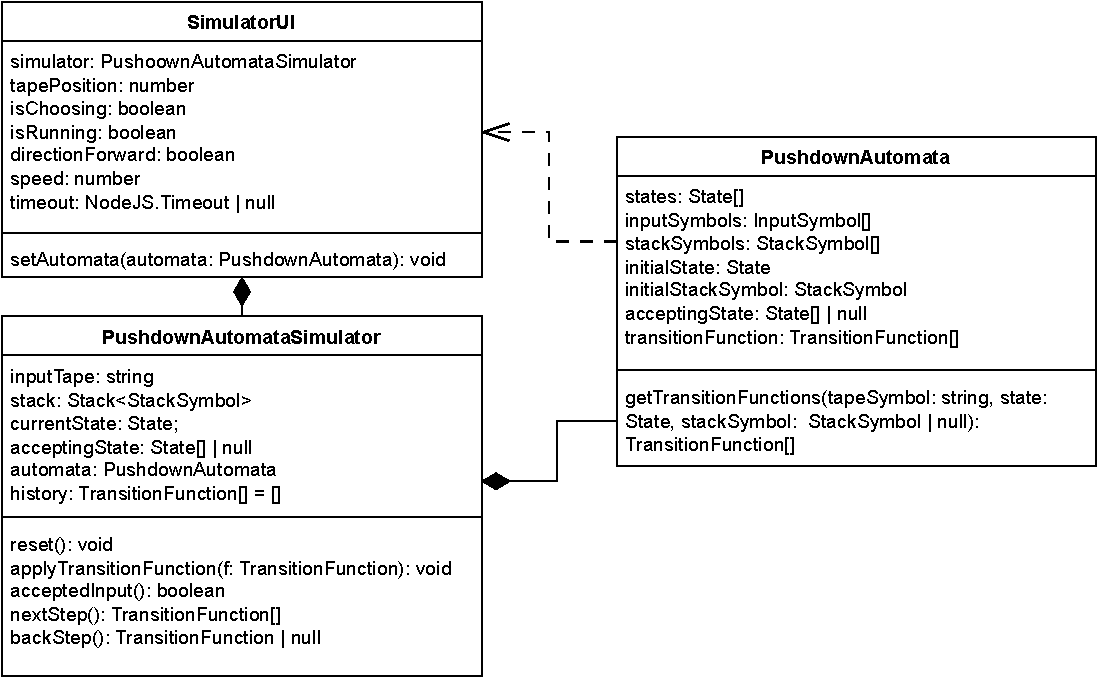
\includegraphics[width=\textwidth]{Figures/SimulatorClasses.drawio.pdf}
    \caption{Třídní diagram tříd simulátoru}\label{fig:SimulatorClasses}
\end{figure}

Nejrozsáhlejší třídou simulátoru je pak třída \texttt{SimulatorUI}.\ Na Obrázku~\ref{fig:SimulatorClasses} jsou jen některé její atributy a metody této třídy. Kromě nich dále obsahuje spoustu atributů, které si ukládají odkazy na jednotlivé části UI, a metody, pomocí kterých jde s UI manipulovat. Díky tomuto může tato třída obstarávat vše, co uživatel vidí a udělá.

Když se uživatel přepne na stránku simulátoru, jako první se zavolá metoda \texttt{setAutomata}. Ta~nastaví simulátor s uživatelem vybraným zásobníkovým automatem a zresetuje celé UI, což obnáší vyčištění vstupní pásky, zásobníku a řídící jednotky, historie použitých přechodů a nastavení výchozích hodnot z automatu. Dále se nastaví výchozí hodnoty proměnných atributů pro automatickou simulaci --- \texttt{isChoosing}, \texttt{isRunning}, \texttt{directionForward}, \texttt{speed} a \texttt{timeout}. Nakonec se~otevře vyskakovací okno pro zadání slova na vstupní pásku. Toto okno obsahuje jednoduchý formulář s~pouze jediným vstupem, nad kterým při každé změně proběhne kontrola, zda obsahuje pouze symboly vstupní abecedy. Když uživatel vstup potvrdí, znovu se zkontroluje, zresetuje se UI a vstup se nastaví do vstupní pásky.

K ovládání uživateli slouží 5 tlačítek a posuvník, Obrázek~\ref{fig:SimulatorButtons}. Krajní tlačítka slouží k zapnutí automatické simulaci. Středové tlačítko slouží k pozastavení automatické simulace a posuvník níže slouží k nastavení času mezi jednotlivými kroky (svou hodnotu ukládá do atributu \texttt{speed}). Zbylé dvě tlačítka slouží k manuálnímu krokování simulace.

\begin{figure}[h]
    \centering
    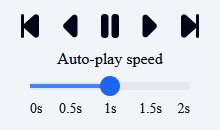
\includegraphics{Figures/PrntScrn_SimulatorButtons.png}
    \caption{Ovládací tlačítka simulátoru}\label{fig:SimulatorButtons}
\end{figure}

Pokud uživatel zmáčkne tlačítko pro krok dopředu, jako první se zkontroluje, zda aktuálně nevybírá přechod. K tomu slouží atribut \texttt{isChoosing}. Pokud je aktuálně v tomto výběru a chce udělat krok vpřed, je na to upozorněn probliknutím oblasti s výběrem přechodu. Pokud v tomto výběru nebyl, pomocí metody \texttt{nextStep} třídy \texttt{PushdownAutomataSimulator} se zjistí všechny přechody, které je možné pro další krok použít. Podle počtu navrácených přechodů mohou nastat tři situace:
\begin{itemize}
    \item Pokud metoda nevrátila žádný přechod, pozastaví se automatická simulace, pokud byla zapnuta, a vyhodnotí se, zda byl vstup přijat.
    \item  Pokud metoda vrátila právě jeden přechod, je tento přechod použit. Pokud byla zapnuta automatická simulace, což se zjistí podle atributu \texttt{isRunning}, nastaví se automatické zapnutí dalšího kroku podle aktuální hodnoty atributu speed a uloží se do atributu \texttt{timeout}.
    \item Pokud metoda vrátila více přechodů, nastaví se atributu \texttt{isChoosing} na \texttt{true} a vygenerují se tlačítka se všemi možnostmi.
\end{itemize}

Když je použit přechod, musí se provést postupně několik věcí. Nejprve se změní vnitřní stav simulátoru metodou \texttt{applyTransitionFunction}. Následně se změní stav řídící jednotky. Pokud byl přečten symbol ze vstupní pásky (nebyl to epsilon přechod), spustí se funkce \texttt{moveTape}. Ta~inkrementuje hodnotu atributu \texttt{tapePosition} a změní styly přilehlý symbolů --- přečtený dostane světlejší barvu a následující symbol dostane barvu tmavší. To umožní uživateli jednodušeji poznat, kterým symbol bude čtený v dalším kroku. Následně se odebere vrchní symbol ze zásobníku a přidají se symboly nové, pokud je přechod obsahuje. Poté se uloží nový záznam do historie. Nakonec~se ještě zkontroluje, jestli již nebylo slovo zásobníkovým automatem přijato.

Pokud bylo možné použít více než jeden přechod, generují se tlačítka pro jednotlivé přechody, Obrázek~\ref{fig:TransitionFunctionChoosing}. Pro každé tlačítko je přidán event, který se spustí po kliknutí. Použije se konkrétní přechod a pokud byla zapnuta automatická simulace, nastaví se automatické zapnutí dalšího kroku podle aktuální hodnoty atributu \texttt{speed} a uloží se do atributu \texttt{timeout}.

Pokud uživatel zmáčkne tlačítko pro krok dozadu, jako první se zkontroluj, zda uživatel zrovna nevybírá přechodovou funkci. Pokud ano, výběr se schová. Pokud ne, získá se z historie poslední použitý přechod a náležitě se upraví stav simulátoru. Jestliže je zapnutá automatická simulace, nastaví se automatické zapnutí předchozího kroku podle aktuální hodnoty atributu \texttt{speed} a uloží se do atributu \texttt{timeout}. Ve chvíli, kdy je historie prázdná, nachází se simulátor ve výchozím stavu a pokud je zapnutá automatická simulace, vypne se.

\begin{figure}[h]
    \centering
    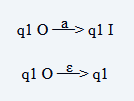
\includegraphics{Figures/PrntScrn_TransitionFunctionChoosing.png}
    \caption{Volba následujícího přechodu}\label{fig:TransitionFunctionChoosing}
\end{figure}

\section{Úložiště}

V kapitole~\ref{chap:AppSpecifications} bylo specifikováno, že si aplikace bude ukládat veškeré automaty, aby se k nim mohl uživatel kdykoliv vrátit. K tomu aplikace využívá local storage.~\cite{LocalStorage} Local storage je úložiště v prohlížeči, které umožňuje ukládat data na straně klienta. Tyto data jsou ukládaná ve formě \texttt{key-value}, kdy pro každý klíč existuje jedna hodnota. Na rozdíl od session storage, kdy dochází k vymazání dat po opuštění stránky, zde data zůstávají i po opuštění stránky nebo zavření prohlížeče.~\cite{Obaseki2020}

V mé aplikaci jsem si pro práci s tímto úložištěm udělal třídu \texttt{Storage}, zkrácený zápis lze vidět ve zdrojovém kódu~\ref{src:StorageClass}. Jelikož local storage umožňuje ukládat klíče a hodnoty pouze jako textové řetězce, udělal jsem si nejprve metody \texttt{Storage}, která hodnotu převede na text a uloží ji do úložiště, a \texttt{load}, která pro zadaný klíč načte hodnotu z úložiště a převede ji z textu zpět na zadaný datový typ nebo objekt. Pro převody používám javascriptové funkce \texttt{JSON.stringify()} a \texttt{JSON.parse()}. Dále jsem si vytvořil metodu \texttt{saveAutomata}, která si nejprve ověří, zda už neexistuje v úložišti záznam se stejným klíčem pomocí metody \texttt{keyExist}. Pokud existuje, zeptá se uživatele, zda tento záznam může přepsat. Následně pomocí metody \texttt{save} uloží automat. Metoda \texttt{loadAutomata} si načte pro~zadaný klíč automat z úložiště funkcí \texttt{load}, nastaví mu správný prototype a vrátí ho návratovou hodnotou. 

\begin{lstlisting}[label=src:StorageClass, caption={Třída Storage}]
    class Storage{
        save<T>(key: string, item: T);
        load<T>(key: string): T | null;
        saveAutomata(key: string, automata: PushdownAutomata): boolean;
        loadAutomata(key: string): PushdownAutomata | null;
        delete(key: string);
        keyExists(key: string): boolean;
        loadFile(e: SubmitEvent);
        insertRow(key: string);
        printAutomatas();
        showAutomata(key: string);
    }
\end{lstlisting}

Metoda \texttt{printAutomatas} slouží k výpisu všech automatů uložených v paměti. Metoda iteruje skrze všechny klíče v úložišti a volá pro ně metodu \texttt{insertRow}. Ta si pro zadaný klíč načte automat z úložiště a uloží nový řádek do tabulky i se všemi příslušnými tlačítky a nastavenými událostmi:
\begin{itemize}
    \item Zobrazení specifikace automatu --- metoda \texttt{showAutomata}
    \item Editace automatu
    \item Spuštění simulátoru
    \item Stažení automatu jako soubor typu JSON (JavaScript Object Notation)
    \item Odstranění automatu z úložiště --- metoda \texttt{delete}
\end{itemize}


Poslední důležitou metodou je metoda \texttt{loadFile} sloužící k nahrání automatu ze souboru. Tato metoda je nastavená jako submit event, spustí se tedy pouze při odeslání formuláře. Formulář obsahuje pouze dvě pole. První je textové a slouží pro pojmenování automatu. Toto jméno se~zobrazuje ve výpisu všech automatů a zároveň je použito jako klíč pro ukládaní. Druhé pole pak~slouží pro nahrání souboru. Po odeslaní se formuláře se spustí metoda \texttt{loadFile}, která nejprve zkontroluje, že jsou obě pole vyplněné. Následně si pomocí metody \texttt{keyExists} zjistí, jestli klíč již není náhodou použit a případně se uživatele zeptá, zda chce automat pro ten klíč přepsat. Poté se ze souboru pokusí vytvořit objekt typu \texttt{PushdownAutomata} a provede se kontrola, zda je automat správně nadefinován, pomocí funkce \texttt{checkPushdownAutomata}. Pokud se nevyskytla žádná chyba, uloží automat do úložiště a přepne uživatele do simulátoru s nastaveným aktuálně nahraným zásobníkovým automatem.

\section{Stránka pro tvorbu zásobníkových automatů}\label{sec:PDABuilderImplementation}

Třída \texttt{formAutomataBuilder} slouží k obsluze stránky, která slouží k tvorbě zásobníkového automatu. Obsahuje metody, které se starají o zpracování dat při odeslání formulářů, kontroly dat, zobrazování chybových hlášek a další. Stránka se skládá z několika částí, kdy každá část odpovídá jedné části zásobníkového automatu. 

První částí je formulář pro přidávání stavů. Po jeho odeslání se přidá nový stav do množiny stavů a přidá se jako jedna z možností, kterou lze vybrat jako přijímací stav a jako počáteční stav. Pokud je stav odstraněn, musí se odstranit i jako možnost v obou výběrech. Další částí je formulář pro přidávání symbolů vstupní abecedy. Po odeslání se symbol uloží do množiny symbolů vstupní abecedy. Po ní následuje formulář pro přidání symbolů zásobníkové abecedy. Ten po odeslání kromě uložení symbolu ještě symbol přidá do seznamu možností počátečního zásobníkového symbolu. Všechny tyto tři formuláře zároveň přidávají tlačítka do části pro tvorbu přechodové funkce. 

Následující dvě části jsou seznamy pro výběr počátečního stavu a počátečního zásobníkového symbolu. Oba tyto seznamy reagují na jakoukoliv změnu díky nastavené change události a vždy si uloží vybranou možnost. Předposlední část slouží k určení, jestli automat bude slovo přijímat prázdným zásobníkem nebo množinou přijímacích stavů. To uživatel může určit pomocí zaškrtávacího pole. Pokud pole není zaškrtnuté, zobrazí se uživateli seznam stavů a uživatel si může vybrat, které stavy budou přijímací.

Poslední část stránky slouží k definování přechodů přechodové funkce. Každý přechod se skládá z 5 částí, které můžeme vidět na Obrázku~\ref{fig:FilledTransition} v prvním řádku. První 4 části jsou povinné, zatímco poslední část může zůstat prázdná dle definice přechodové funkce. Při kliknutí na kteroukoliv část se na druhém řádku zobrazí všechny možnosti, které mohou být použity pro danou část. Zobrazují se zde vždy jen symboly, které byly přidány dříve, ale pro vstupní symbol je zde ještě přidán symbol $\varepsilon$. Při kliknutí tlačítka \texttt{Add transition} se zkontroluje, že jsou první 4 části vyplněné, že~přechod obsahuje pouze symboly nadefinovaných abeced a nadefinované stavy a zda tento přechod již neexistuje. Pokud je vše v pořádku, tak přidá přechod do množiny přechodů přechodové funkce.

\begin{figure}[h]
    \centering
    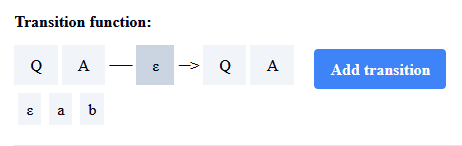
\includegraphics{Figures/PrntScrn_FilledTransition.png}
    \caption{Vyplněný přechod na stránce tvorby zásobníkového automatu}\label{fig:FilledTransition}
\end{figure}

Při kliknutí na tlačítko \texttt{Save} automata ve spodní části stránky se spustí funkce \texttt{saveEventHandler}. Ta jako první zkontroluje, že všechny abecedy mají minimálně jeden symbol, množina stavů alespoň jeden stav a že uživatel vybral počáteční stav a počáteční zásobníkový symbol. Dále zkontroluje, zda se jedná o automat přijímající prázdným zásobníkem nebo přijímajícími stavy a zda je případně vybrán alespoň jeden stav. Poté ještě zkontroluje, zda je nadefinován alespoň jeden přechod přechodové funkce. Následně se provede kontrola celého zásobníkového automatu pomocí funkce \texttt{checkPushdownAutomata}, která je podrobněji popsána v podkapitole~\ref{sec:checkPushdownAutomata}. Pokud se nikde nevyskytla chyba, automat se uloží do úložiště a stránka se přepne do simulátoru.

\section{Funkce checkPushdownAutomata pro kontrolu automatu}\label{sec:checkPushdownAutomata}

Poslední důležitou částí implementace je funkce pro kontrolu definice zásobníkových automatů. Tato funkce se volá při nahrání zásobníkového automatu ze souboru nebo při jeho definici přímo na stránce. Funkce postupně prochází jednotlivé části automatu a kontroluje jejich správnost. V~případě nalezené chyby si uloží chybovou hlášku a na konci je všechny vypíše uživateli.

Jako první postupně zkontroluje množinu stavů a vstupní a zásobníkovou abecedu. U všech tří kontroluje, jestli množiny nejsou prázdné a zda neobsahují duplicity. Jelikož typescript neobsahuje datový typ \texttt{char}, ale pouze \texttt{string}, tak u abeced ještě zkontroluje, že všechny symboly jsou délky jednoho znaku.

Dále se kontroluje počáteční stav a počáteční zásobníkový symbol. U obou se zkontroluje, zda jsou součástí konkrétních množin. Pokud automat přijímá množinou přijímacích stavů, tak se pro každý přijímací stav taktéž zkontroluje, zda je součástí množiny stavů. 

Nakonec se kontrolují přechody přechodové funkce. Pro každý přechod se zkontroluje, zda všechny jeho části (oba stavy, zásobníkové symboly a symbol vstupní abecedy, pokud není $\varepsilon$) jsou součástí konkrétních množin.

Nakonec se zkontroluje, jestli pole chybových hlášek je prázdné. Pokud není, tak se pomocí funkce \texttt{alert} zobrazí všechny chybové hlášky, viz Obrázek~\ref{fig:PDACheckErrors}, a funkce vrátí hodnotu \texttt{false}. V~opačném případě vrátí funkce hodnotu \texttt{true}.

\begin{figure}[h]
    \centering
    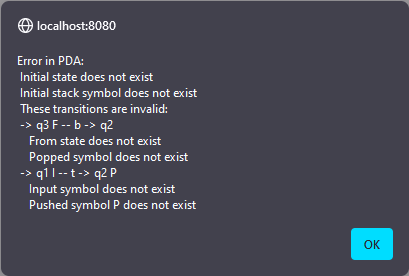
\includegraphics[width=0.6\textwidth]{Figures/PrntScrn_PDACheckErrors.png}
    \caption{Ukázka chybových hlášek kontroly zásobníkového automatu}\label{fig:PDACheckErrors}
\end{figure}

\endinput